\section{Einführung}

Sei $M$ eine glatte Abbildung, $f: M \to \R$ eine glatte Abbildung, 
$a \in \R$. Dann ist $M^a = f^{-1}(- \infty, a]$ ein \textit{sublevel set} von 
$f$. Das Ziel des Vortrags ist es, die Topologie der sublevel sets einer 
Abbildung mit ausschließlich nicht degenerierten kritischen Punkten, so genannten
\textit{Morsefunktionen}, zu verstehen.
Wir Untersuchen die Situation anhand des Torus. Wir stellen uns Morsefuinktionen
der einfachheitshalber als "Höhenfunktionen" vor.

\begin{figure}[H]
    \centering
    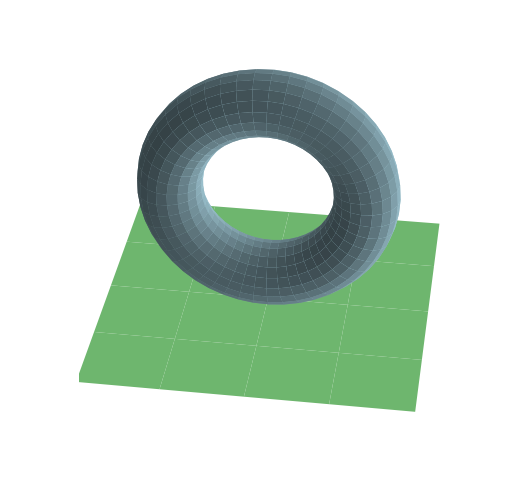
\includegraphics[width=0.6\linewidth]{resources/Me-Diagram1-torus-plane.png}
    \label{fig:me-diagram1}
    \caption{Torus auf der Ebene}
\end{figure}

Es sei $f$ die Abbildung vom Torus nach $\R$, die jedem Punkt den minimalen
Abstand zu der eingezeichneten Ebene zuordnet. 
Die kritischen Punkte dieser Höhenfunktion sind $p$, $q$, $r$ und $s$.
Man stellt sich vor, dass man den Torus nach und nach mit Wasser befüllt. Dann 
ist für $a \in \R$ $M^a = f^{-1}(-\infty, a]$ die Menge der Punkte die bei der
Wasserhöhe $a$ das Wasser berühren. 

\begin{itemize}
    \item Für $a < 0$ ist $M^a = \varnothing$.
    \item Für $0 \leq a < f(p)$ ist $M^a$ homotopieäquivalent zum Punkt.
    \item Für $f(p) \leq a < f(q)$ ist $M^a$ homotopieäquivalent zum Kreis,
        an dem ein "Henkel" befestigt wurde.
    \item Für $f(q) \leq a < f(r)$ ist $M^a$ Homotopieäquivalent zum Zyliner,
        an dem ein "Henkel" befestigt wurde.
    \item Für $f(s) \leq$ ist $M^a$ der Torus selbst.
\end{itemize}

Wir bemerken: 
\begin{itemize}
    \item Gibt es im Intervall $[a, b]$ keine kritischen Werte, so haben alle
        $M^c$ für $c \in [a, b]$ denselben Homotopie-Typ
    \item Gibt es im Intervall $[a, b]$ genau einen kritischen Wert $c$ und ist
        $ \#f^{-1}(p) = 1$, dann hat $M^b$ den Homotopie-Typ von $M^a$ mit einem 
        Henkel angebracht (Was auch immer das bedeutet).
\end{itemize}

Um diese zwei Aussagen zu präzisieren, brauchen wir einige Definitionen:

\begin{definition}[Deformationsretrakt]
    Sei $X$ ein topologischer Raum und $A \subseteq X$ ein Unterraum von $X$.
    Eine stetige Abbildung $r: X \times [0, 1] \rightarrow X$ heißt 
    \textit{Deformationsretraktion} auf $A$, falls gelten:
    \begin{align*}
        & r(\cdot, 0) = \id_X \\
        & r(X, 1) \subseteq A \\
        & r(\cdot, 1)|_A = \id_A \\
    \end{align*}
    $A$ heißt \textit{Deformationsretrakt}, falls eine Deformationsretraktion
    von $X$ auf $A$ existiert.
\end{definition}

Deformationsretrakte haben einige schöne Eigenschaften. Falls $A$ ein
Deformationsretrakt von $X$ ist, so ist die Inklusion $A \rightarrow X$ eine
Homotopieäquivalenz. Da Homotopieäquivalenz transitiv ist, hat ein weiterer
Deformationsretrakt $B$ von $X$ deshalb denselben Homotopietypen wie $A$. \\
Es eine Tatsache, dass zwei Unterräume $A$ und $B$ genau dan denselben 
Homotopietypen haben, wenn sie beide Deformationsretrakte eines gemeinsamen 
Oberraumes sind. Um dies einzusehen benötigt man weitere topologische 
Theorie.

\begin{definition}[Eine $k$-Zelle anbringen]
    Es sei $X$ ein Topologischer Raum. Seien
    \[ e^k = D^k = \{(x_1, ..., x_k) \in \R^k: x_1^2 + ... + x_k^2 \leq 1\} \]
    \[ \varphi: \del e^k \rightarrow X \text{ stetig } \]
    \[ X \cup_{\varphi} e^k = (X \amalg e^k) / \sim, \text{ wobei } \]
    \[ \del e^k \ni x \sim y \in X \Leftrightarrow \varphi(x) = y \]
    Dann heißt $e^k$ $\lambda$-Zelle, $\varphi$ Anheftungsabbildung 
    und $X \cup_{\varphi} e^k$ heißt $X$ mit einer $k$-Zelle 
    angebracht.
\end{definition}

\textbf{ZEICHNUNG 1-Zelle, 2-Zelle}

Ein Paar Beispiele: 
\begin{itemize}
    \item Eine $0$-Zelle in einen nichtleeren Raum anzubringen 
        verändert diesen nicht, und
        \[\varnothing \cup_{\varphi} e^0 = \ast\]
    \item Eine $1$-Zelle lässt uns Zusammenhangskomponenten mit einer "Schnur"
            verbinden, oder ist das Anheften einer "Schlaufe".
    \item Eine $2$-Zelle anzubringen kann sein wie das anbringen einer Blase oder
        das stopfen eines Loches durch eine "Membran".
\end{itemize}

Eine $k$-Zelle kann also zwei Sachen: "Löcher", die von der $k$-ten Homologie
"gemessen" werden zu erschaffen oder "Löcher", die von der $(k-1)$-ten Homologie
"gemessen" werden zu "stopfen". Wenn wir also unsere Mannigfaltigkeit in 
Bezug auf solche Zellen bringen können, dann macht es uns das leichter die 
Topologie (und Homologie) der Mannigfaltigkeit besser zu verstehen. Wenn wir
sogar die gesamte Mannigfaltigkeit durch iteratives anbringen von $k$-Zellen
an den leeren Raum "erschaffen" können, dann können wir einigen Aussagen über 
die Homologie des Raumes machen. 


\begin{theorem}[Erstes Deformationslemma]
    \label{theorem:erstes deformationslemma}
    Es sei $M$ eine glatte Mannigfaltigkeit und $f: M \rightarrow \R$ eine
    glatte Abbildung. Hat $f$ keine kritischen Werte im Intervall [a, b] und ist
    $f^{-1}[a, b]$ kompakt, so existiert ein Diffeomorphismus 
    $M^a \rightarrow M^b$, und $M^a$ ist ein Deformationsretrakt von $M^b$.
\end{theorem}

\begin{theorem}[Zweites Deformations-Lemma]
    \label{theorem:zweites deformationslemma}
    Es sei $M$ eine glatte Mannigfaltigkeit, $f: M \rightarrow \R$ eine glatte
    Abbildung und $p$ ein nicht-degenerierter kritischer Punkt mit Index 
    $k$. Sei $c := f(p)$ und $\varepsilon \geq 0$, sd. 
    $f^{-1}[c - \varepsilon, c + \varepsilon]$ kompakt ist und außer $p$ keine 
    weiteren kritischen Punkte von $f$ beinhaltet. Dann hat $M^{c-\varepsilon}$
    denselben Homotopietypen wie $M^{c - \varepsilon} \cup_{\varphi} e^k$
    für eine Anheftungsabbildung 
    $\varphi: \del e^k \rightarrow M^{c-\varepsilon}$
\end{theorem}
